\begin{frame}{Selected Alternatives to \alert{The Things Network}}
    \begin{columns}[onlytextwidth]
        \begin{column}{0.15\textwidth}
            
\includegraphics[width=2cm]{material/helium_logo.png}
        \end{column}
        \begin{column}{0.85\textwidth}
        \begin{itemize}
            \item Decentralized wireless network for IoT devices.
            \item Uses blockchain to incentivize network coverage.
        \end{itemize}
        \end{column}
    \end{columns}

    \vspace{0.5cm}

    \begin{columns}[onlytextwidth]
        \begin{column}{0.15\textwidth}
            
\includegraphics[width=2cm]{material/loriot_logo.png}
        \end{column}
        \begin{column}{0.85\textwidth}
        \begin{itemize}
            \item Global LoRaWAN network provider for professional applications.
            \item Offers private and public network deployment options.
        \end{itemize}
        \end{column}
    \end{columns}

    \vspace{0.5cm}

    \begin{columns}[onlytextwidth]
        \begin{column}{0.15\textwidth}
            
\includegraphics[width=2cm]{material/actility_logo.png}
        \end{column}
        \begin{column}{0.85\textwidth}
        \begin{itemize}
            \item Focuses on large-scale LoRaWAN deployments.
            \item Offers network management, IoT application enablement, and more.
        \end{itemize}
        \end{column}
    \end{columns}

    \vspace{0.5cm}

    \begin{columns}[onlytextwidth]
        \begin{column}{0.15\textwidth}
            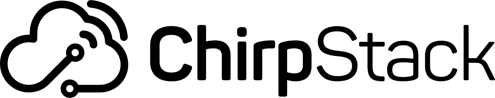
\includegraphics[width=2cm]{material/chirpstack_logo.png}
        \end{column}
        \begin{column}{0.85\textwidth}
        \begin{itemize}
            \item Open-source LoRaWAN Network Server stack.
            \item Provides flexibility for deploying private LoRaWAN networks.
            \item Suitable for enterprise and industrial IoT applications.
        \end{itemize}
        \end{column}
    \end{columns}
\end{frame}
